\subsection{Minority allocation and the eight-expression follow-up}\label{sec:new-results}
Preserving target probability values does not preserve the selective result. Distance-selected seven-output Soft has mean disagreement of 23.68\%, compared with 24.48\% for Permutation: a difference of $-0.794$ pp, with a conditional 95\% interval of $[-1.071,-0.474]$. The three paired differences are $-0.523$, $-0.935$ and $-0.924$ pp (sample SD 0.235 pp). At epoch 12, the mean remains negative ($-0.548$ pp, interval $[-0.855,-0.261]$). Thus, the observed minority allocation performs better than this particular entropy- and maximum-preserving permutation. The control changes aggregate class priors, so the comparison does not uniquely isolate category identity from those priors.

The principal eight-output comparison gives Soft 23.74\% disagreement, Uniform 24.58\% and Tie-Uniform 23.79\%. Soft minus Uniform is $-0.836$ pp, interval $[-1.152,-0.509]$, with paired differences $-0.454$, $-1.191$ and $-0.863$ pp (SD 0.369 pp). This contrast remains negative at epoch 12 ($-0.385$ pp) and under risk-based checkpoint selection ($-0.585$ pp). In contrast, Soft minus Tie-Uniform is only $-0.052$ pp, interval $[-0.314,+0.212]$. Its epoch-12 and risk-selected means are $-0.130$ and $-0.104$ pp, respectively; both intervals also cross zero. These intervals do not establish equivalence. Figure~\ref{fig:followup-contrasts} retains all eight planned contrasts, rather than only the larger differences against Uniform.

\begin{figure}[!htbp]
\centering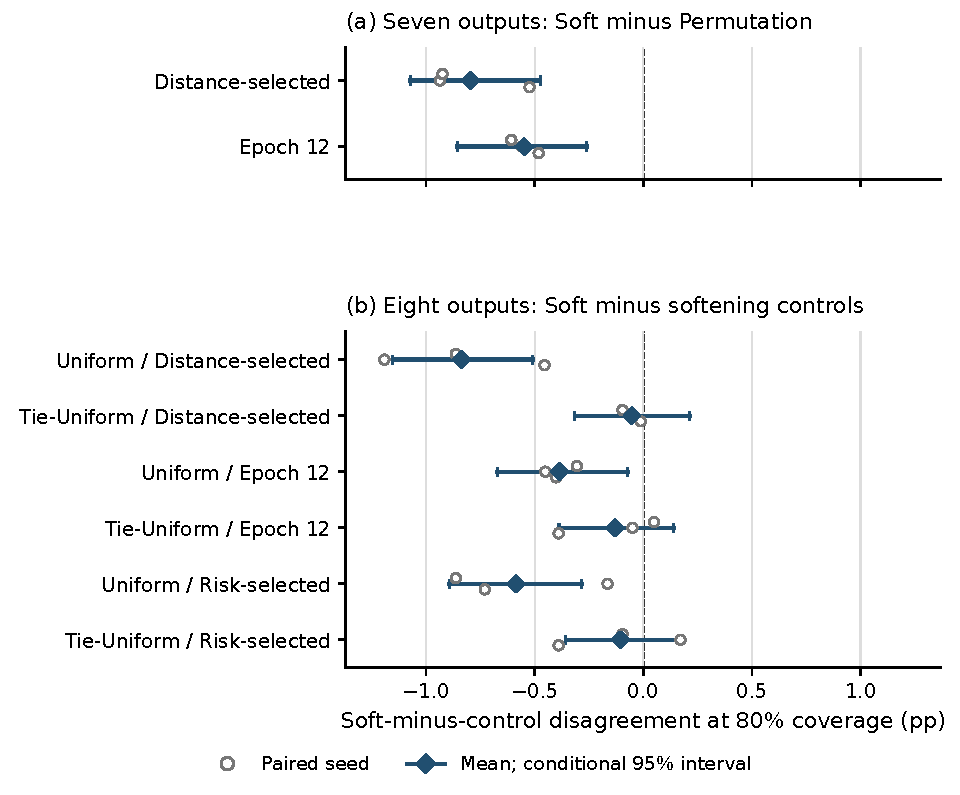
\includegraphics[width=\linewidth]{final_revision_2026_10_20/source/figures/FollowupContrasts.pdf}
\caption{Final adaptive follow-up at 80\% own-MSP coverage. Hollow symbols show three paired-seed differences, diamonds their mean, and bars conditional 95\% exact-pixel-cluster intervals. (a) Seven-output Soft minus Permutation. (b) Eight-output Soft minus Uniform or Tie-Uniform under all three checkpoint rules. Negative favors Soft. Distance selection is the principal rule; fixed epoch and risk selection are sensitivities. Different rules can select the same weights, and intervals do not represent uncertainty over new training seeds}\label{fig:followup-contrasts}
\end{figure}

Full-coverage distributional agreement remains more consistent. Eight-output Soft has lower ten-category squared distance than both softening controls in every seed and checkpoint rule. Distance-selected means are 0.09467 for Soft, 0.11708 for Uniform and 0.10962 for Tie-Uniform. However, expanding the vocabulary does not by itself establish a selective improvement: the seven- and eight-output Soft means are 23.68\% and 23.74\% on their separately accepted sets. This policy comparison changes supported weights, classifier dimension and fitted predictions together.

The new fixed-image comparisons also distinguish predictor changes from selection changes. For distance-selected eight-output models, Soft minus Uniform is $-0.729$ pp on Soft's accepted images and $-0.132$ pp on Uniform's images. Soft minus Tie-Uniform changes sign: $-0.279$ pp on Soft's images and $+0.125$ pp on Tie-Uniform's. The corresponding seven-output Soft-minus-Permutation means are $-0.523$ pp on Soft's set and $-0.074$ pp on Permutation's. These are means on identical images within each selector, not a causal decomposition of the own-ranking differences.

The separately frozen ranking extension reinforces the distinction. Calibration chose MSP over centered normalization for every new state, as it had for the original 48 states. For distance-selected eight-output Soft minus Tie-Uniform, the mean changes from $-0.052$ pp with MSP to $+0.280$ with margin, $+0.164$ with negative entropy and $+0.131$ with centered normalization. Predictions are unchanged; the accepted images change. Soft minus Uniform remains negative under these distance-selected scores, but its epoch-12 margin contrast is approximately zero ($+0.003$ pp). Supplementary Sect.~S11 retains every new state, seed, selected epoch, fixed-image comparison and ranking sensitivity. The findings support a conditional benefit against specific controls, not a score-independent advantage from retaining the full vote distribution.
